%%%%%%%%%%%%%%%%%  Debut du fichier Latex  %%%%%%%%%%%%%%%%%%%%%%%%%%%%%%
\documentclass[12pt,onecolumn]{article}
%\usepackage[style=numeric,maxnames=1,uniquelist=false]{biblatex}
%\usepackage[backend=bibtex,style=numeric,minnames=4,maxnames=4,firstinits=true,sorting=none]{biblatex} 
\usepackage[backend=bibtex,bibstyle=phys,citestyle=authoryear,maxcitenames=1,minbibnames=3,maxbibnames=3,giveninits=true,natbib,doi=false,isbn=false]{biblatex} 
%\usepackage[authordate,bibencoding=auto,strict,backend=biber,natbib]{biblatex}

 %backend=biber is 'better'  
\makeatletter
\def\blx@maxline{77}
\makeatother
\renewbibmacro{in:}{} % to not have the "In:" to indicate the review
\AtEveryBibitem{\clearfield{title}} % to remove the titles in the biblio
% no page info
\AtEveryBibitem{%
  \ifentrytype{article}{%
    \clearfield{pages}%
  }{%
  }%
}
% no language info
\AtEveryBibitem{\clearlist{language}}
% no language no page
\AtEveryBibitem{%
  \clearfield{volume}%
  \clearfield{number}}
% To avoid parenthesis if no year entry in bib file
\renewbibmacro*{issue+date}{%
  \ifboolexpr{not test {\iffieldundef{year}} or not test {\iffieldundef{issue}}}
    {\printtext[parens]{%
       \iffieldundef{issue}
         {\usebibmacro{date}}
         {\printfield{issue}%
          \setunit*{\addspace}%
          \usebibmacro{date}}}}
    {}%
  \newunit}


\ExecuteBibliographyOptions{isbn=false,url=false,doi=false,eprint=false}

%\bibliography{/Users/Ileyk/Documents/Bibtex/Hubble_fellowship_no_url} 
\addbibresource{/Users/Ileyk/Documents/Bibtex/CNRS_19_fixed.bib}
%%% Pour un texte en francais


%%\usepackage[applemac]{inputenc}
%\usepackage[francais]{babel}
	         % encodage des lettres accentuees
\usepackage[T1]{fontenc}
\usepackage[utf8]{inputenc}          % encodage des lettres accentuees
%\usepackage{graphicx}
%%\usepackage{graphicx} \def\BIB{}
\usepackage[paper=a4paper,left=2.5cm,right=2.5cm,top=3.5cm,bottom=3.5cm]{geometry}
\usepackage{multicol}
\usepackage{graphicx,wrapfig,lipsum} 
%\def\BIB{}
\usepackage{caption}
\usepackage{subcaption}
\usepackage[pdftex]{hyperref}
%\usepackage{natbib}
\usepackage{url}
\usepackage{perpage} %the perpage package
\MakePerPage{footnote} %the perpage package command
\hypersetup{
    colorlinks,%
    citecolor=black,%
    filecolor=black,%
    linkcolor=black,%
    urlcolor=blue     % can put red here to visualize the links
}

\usepackage{enumitem}
\usepackage{amssymb}

%\renewcommand{\refname}{}

\usepackage{floatrow}

\usepackage{fancyhdr}
\usepackage{lastpage}

\pagestyle{fancy}
\fancyhf{}
\rhead{Research summary}
\lhead{El Mellah Ileyk}
\rfoot{\thepage / \pageref{LastPage}}

\DeclareUnicodeCharacter{00A0}{ }

\usepackage{xspace}

%%% Quelques raccourcis pour la mise en page
\newcommand{\remarque}[1]{{\small \it #1}}
\newcommand{\rubrique}{\bigskip \noindent $\bullet$ }
\newcommand{\sgx}{SgXB\xspace}
\newcommand{\sgxs}{SgXBs\xspace}
\newcommand{\ulx}{ULX\xspace}
\newcommand{\sfxt}{SFXT}
\newcommand{\sg}{Sg\xspace}
\newcommand{\co}{CO\xspace}
\newcommand{\gw}{GW\xspace}
\newcommand{\gws}{GWs\xspace}
\newcommand{\grb}{GRB\xspace}
\newcommand{\grbs}{GRBs\xspace}
\newcommand{\eos}{EOS\xspace}
\newcommand{\mhd}{MHD\xspace}
\newcommand*{\hmxb}{HMXB\@\xspace}
\newcommand*{\hmxbs}{HMXBs\@\xspace}
\newcommand*{\lmxb}{LMXB\@\xspace}
\newcommand*{\rlof}{RLOF\@\xspace}
\newcommand*{\ns}{NS\@\xspace}
\newcommand*{\nss}{NSs\@\xspace}
\newcommand*{\bh}{BH\@\xspace}
\newcommand*{\bhs}{BHs\@\xspace}
\newcommand*{\eg}{e.g.\@\xspace}
\newcommand*{\ie}{i.e.\@\xspace}
\newcommand*{\aka}{a.k.a. \@\xspace}
\newcommand*\diff{\mathop{}\!\mathrm{d}}
\newcommand{\mystar}{{\fontfamily{lmr}\selectfont$\star$}}
\newcommand*{\msun}{$M_{\odot}$\@\xspace}
\newcommand*{\mdotstar}{$\dot{M}_{\text{\mystar}}$\@\xspace}
\newcommand*{\mdotacc}{$\dot{M}_{\text{acc}}$\@\xspace}
\newcommand*{\ledd}{$L_{\text{Edd}}$\@\xspace}


\newcommand{\ignore}[1]{}

%\renewcommand*\rmdefault{iwona}

%\pagenumbering{gobble}

%\bibliographystyle{abbrvnat}
%\setcitestyle{authoryear,open={((},close={))}}

%\renewcommand{\thefootnote}{\roman{footnote}}

% -------------------------------------------------
\newcommand{\horrule}[1]{\rule{\linewidth}{#1}} % Create horizontal rule command with 1 argument of height

\title{	
\vspace*{-2.5cm}
%\normalfont \tiny 
%%\textsc{Paris Diderot} \\ [25pt] % Your university, school and/or department name(s)
%\horrule{0.5pt} \\[0.4cm] % Thin top horizontal rule
%\Large Speeding up the spinning top\\
%\large How accretion sets the pace in High Mass X-ray Binaries  \\ % The assignment title
%\horrule{2pt} \\[0.5cm] % Thick bottom horizontal rule
}
\author{\tiny} % Your name
\date{\tiny }%\normalsize\today} % Today's date or a custom date
% -------------------------------------------------

%\makeatletter
%\def\@xfootnote[#1]{%
%  \protected@xdef\@thefnmark{#1}%
%  \@footnotemark\@footnotetext}
%\makeatother

%\usepackage[square,numbers,sort]{natbib}
%\usepackage{har2nat} % "natbib" is loaded automatically

%
%\let\oldthebibliography\thebibliography
%\renewcommand{\thebibliography}[1]{%
%  \oldthebibliography{#1}
%  \let\oldbibitem\bibitem
%  \let\oldtextsc\textsc
%  \def\oldbbland{et}
%  \newcounter{authorcount}
%  \def\bibitem[##1]##2{%
%    \let\textsc\oldtextsc
%    \let\bbland\oldbbland
%    \oldbibitem[##1]{##2}%
%    \let\textsc\mytextsc%
%    \let\bbland\mybbland
%    \setcounter{authorcount}{0}
%  }
%  \def\mybbland{\setcounter{authorcount}{0}\oldbbland}
%  \def\dropetal##1.{ \bbletal}
%  \def\mytextsc##1{%
%    \oldtextsc{##1}%
%    \stepcounter{authorcount}%
%    \ifnum\value{authorcount}=2\relax%
%      \expandafter\dropetal%
%    \fi%
%  }%
%}


\begin{document}

%\bibpunct{[}{]}{;}{n}{,}{,}

%%%%%%%%%%%%%%%%%%%%%%%%%  PREMIERE PAGE %%%%%%%%%%%%%%%%%%%%%%%%%%%%%%
%%% DANS CETTE PAGE, ON REMPLACE LES INDICATIONS ENTRE CROCHETS [...]
%%% PAR LES INFORMATIONS DEMANDEES
%%%%%%%%%%%%%%%%%%%%%%%%%%%%%%%%%%%%%%%%%%%%%%%%%%%%%%%%%%%%%%%%%%%%%%%

\renewcommand{\headrulewidth}{1pt}
\pagestyle{fancy}
\fancyhf{}
\rhead{Research proposal}
\lhead{El Mellah Ileyk}
\rfoot{\thepage / \pageref{LastPage}}

\vspace*{-1.2cm}
\begin{center}
\Large \textbf{Kilonovae following compact object coalescences}\\
\large What they tell us about the ultimate moments of merging neutron stars  
\end{center}
\normalfont

The discovery of the first gravitational wave (\gw) signal three years ago marked the dawn of a new astronomy \citep{Abbott2016}. Four decades after the indirect detection by Hulse and Taylor in an inspiralling pulsar binary \citep{Hulse1974}, we are now fully able to capture the very last moments of the epic life of massive stars through the burst of \gw emitted when the compact remnants eventually merge. If the first detections were interpreted as merging black holes (\bhs), without any electromagnetic counterpart, a \gw signal from two merging neutron stars (\nss) was observed last year in association with a short gamma ray burst (\grb) and a subsequent luminous blue kilonova \citep{TheLIGOScientificCollaboration2017}. The crossed analysis of these three signals can unearth unvaluable information on a multitude of aspects : the equation-of-state (\eos) of condensed matter in \nss, the nucleosynthesis of the heaviest elements and new constrains on gravity in the strong field regime are only a few examples of the promising breakthroughs ahead.

Short \grbs are intense non-repeating flares of $10^{51}$ ergs released as gamma-rays over less than 2 seconds \citep{Berger2014}. With the discovery of an X-ray afterglow by \citet{Gehrels2005} came the identification of the host galaxy of a short \grb and the confirmation of their cosmological origin. They have long been thought to be powered by the accretion of a massive remnant disc onto the compact object formed after a \ns-\ns/\bh-\ns merger \citep{Eichler1989}. The interplay between accretion and rapid rotation of the central engine can drive a collimated ultra-relativistic outflow \citep{Piran2005}. Within this jet with typical opening-angles of a few degrees, relativistically beamed gamma-ray emission arises from energy dissipation via internal shocks \citep{Rees1992}. External shocks with circumburst material generate the aforementioned afterglow \citep{Kumar2015}.

Kilonovae are week-long supernovae-like transients, with a spectral peak ranging from near infrared to optical and a peak luminosity at 10$^{40-41}$erg$\cdot$s$^{-1}$ reached after a few days \citep{Tanaka2016,Metzger2017}. \citet{Tanvir2013} and \citet{Berger2013} associated kilonovae and \grbs by finding evidence for a significative near infrared excess in the late-time afterglow of a \grb. Kilonovae are thought to be produced by neutron-rich material ejected during a \ns-\ns/\bh-\ns merger : as the mildly relativistic cocoon expands, it is heated by radioactive decay \citep{Li1998}, a millisecond magnetar \citep{Yu2013} and/or fall-back accretion onto the central body \citep{Rosswog2007}. The relative contribution of these three mechanisms lies at the core of this research proposal whose main scientific questions are :

\begin{enumerate}[itemsep=0mm]
\item How neutron-rich are the different components of the ejecta?
\item How can the rotational energy of a fastly rotating magnetar remnant be transferred to the ejecta?
\item How could material falling back at later times heat the ejecta?
\end{enumerate}

A simplified sketch of the different components is displayed in Figure\,\ref{fig:sketch}. Each of the three next sections describes the proposed research tracks to address these questions. The last section contains a description of the numerical tool and of the compatibility with the scientific projects of the host institution, followed by two conclusive paragraphs.

\begin{figure}[!b]
\vspace*{-0.3cm}
\floatbox[{\capbeside\thisfloatsetup{capbesideposition={right,center},capbesidewidth=8cm}}]{figure}[\FBwidth]
{\caption{Simplified sketch of the different physical components. The central black dot stands for the merger remnant. If it is a \ns, a magnetosphere is expected (green dipole), along with a magnetar wind nebula containing copious amounts of neutrinos ("$\nu$-wind"). Material ejected in the equatorial plane of the fastly rotating remnant might sometimes form a disc from which can depart a neutrino-driven wind. The jets responsible for the short \grb are represented in black (with double lines indicating internal and external shocks). The kilonova (in red) comes from outflowing material. The details of these pictures depend strongly on the initial merger and the nature of the remnant.}\label{fig:sketch}}
{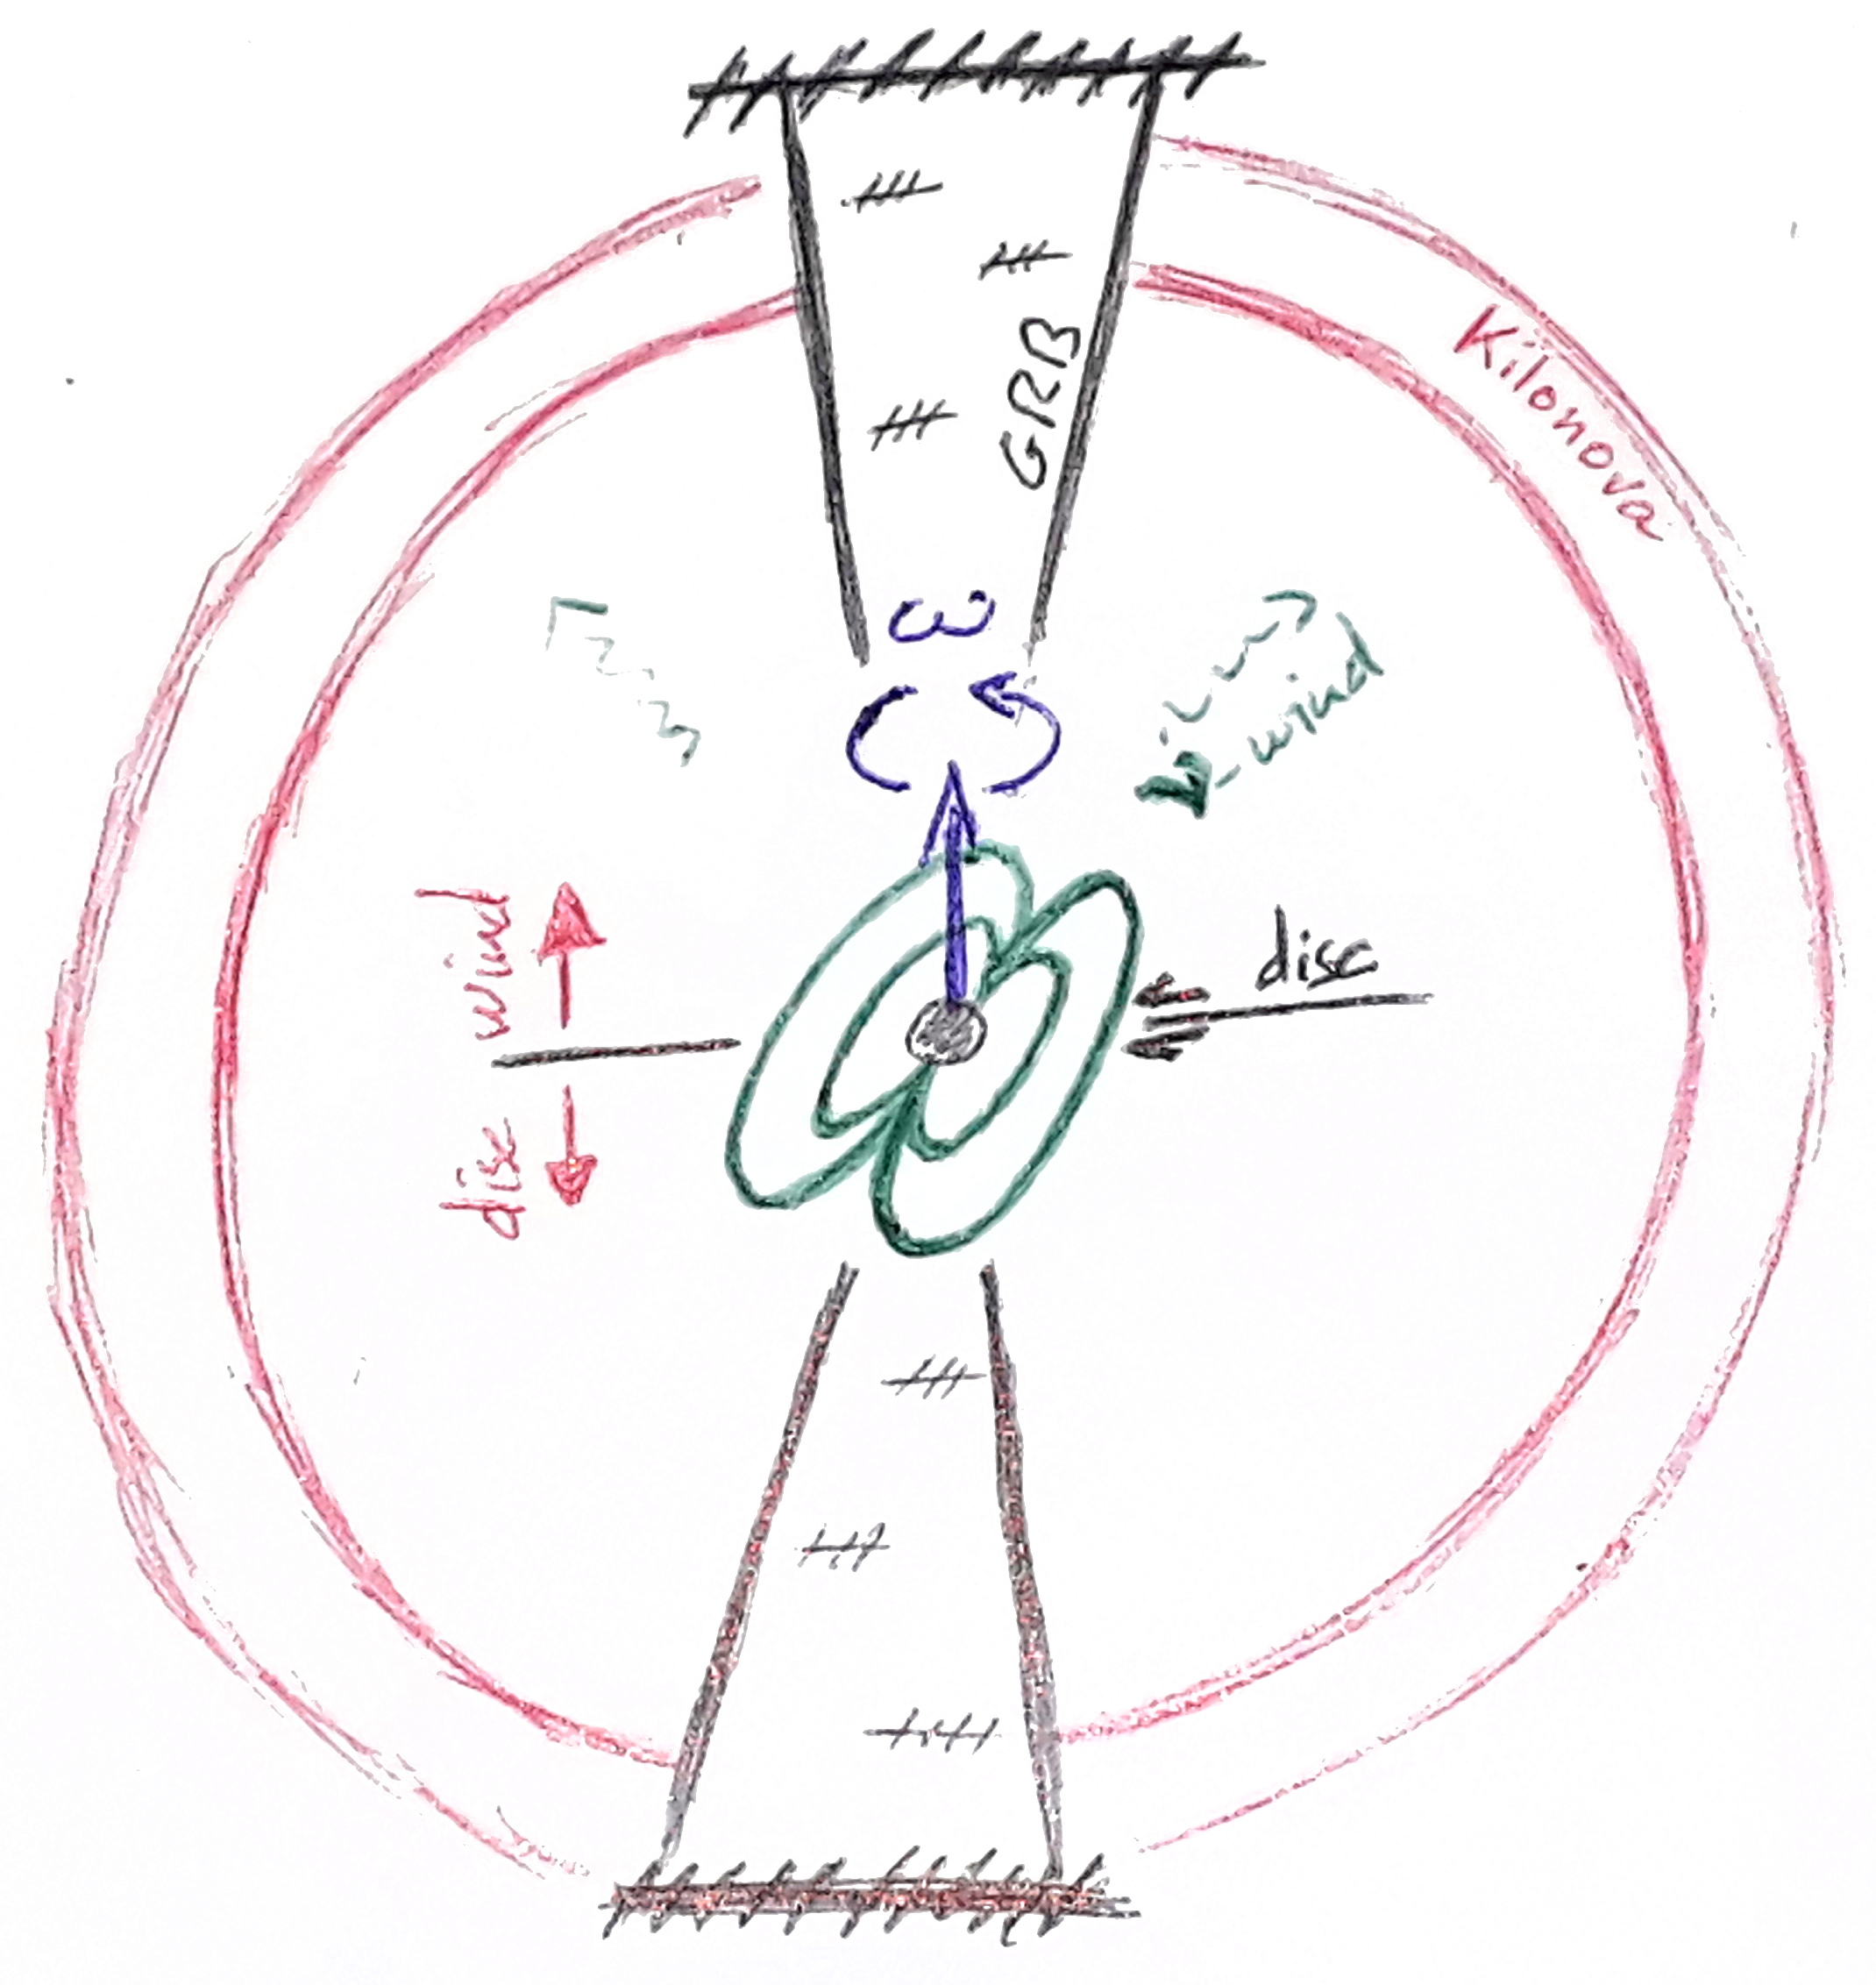
\includegraphics[width=8cm]{Figures/sketch_GRB_kilonova.jpg}}
%\vspace*{-0.4cm}
\end{figure}

\section{A site for nucleosynthesis of neutron-rich elements}

Kilonovae have long been suspected to be the main site for the nucleosynthesis of the heaviest elements \citep{Lattimer1974}, along with core-collapse supernovae \citep{MacFadyen1999}. Due to their dense neutron-rich content (\ie low electron fraction), kilonovae can be the stage of rapid neutron-capture by seed nuclei like Iron, the so-called "r-process". The yield of this nucleosynthesis and the associated heating of the kilonova can be derived from nuclear reaction networks \citep{Metzger2010} and the electron fraction, with higher yields for lower electron fractions. However, the electron fraction can only be deduced once we properly account for neutrino-irradiation : neutrino absorption reactions on nucleons increase the electron fraction of the material and might inhibit the formation of heavy elements such as lanthanides. Since the opacity of lanthanides can quickly dominate and determine the properties of a kilonova light curve, we need to figure out how neutrinos interact with the different components during a \ns-\ns/\bh-\ns merger.

At the LUTh, Micaela Oertel's team developed a computationally affordable method to solve neutrino transport in the context of core-collapse supernovae \citep{Peres2011,Peres2013}. I would like to extend this treatment to \ns-\ns/\bh-\ns mergers and implement it in a form suitable to be used in conjunction with finite volume magneto-hydrodynamics (\mhd) codes such as \texttt{MPI-AMRVAC} (see last section). During my postdoctoral years, I have worked on different schemes to solve the radiative transfer equations : methods inspired from long characteristics with Jon Sundqvist (KU Leuven), flux-limited diffusion and an alternating directional implicit scheme with Nicolas Moens (a PhD student I co-supervise with Jon Sundqvist) and multi-grid solvers with Jannis Teunissen (CWI Amsterdam). Although physical differences exist between neutrinos and photons, these numerical techniques share many common points with the ones developed for neutrino transport. Coupling the micro-Physics to the flow dynamics has become an absolute requirement to improve our understanding of these high temperature environments. Another human asset to connect the heating of the merger surroundings to the observed light curves is the presence of Fr\'{e}d\'{e}ric Vincent for the last couple of years at the LESIA, nearby the LUTh. The general relativity ray-tracing code he led the development of, \texttt{GYOTO} \citep{Vincent2011}, could prove useful to appreciate transport mechanisms in the immediate vicinity of the compact object.

\section{Spinning down of a magnetar remnant}

Extraction of the huge rotational energy contained in a millisecond magnetar (\ie with a magnetic field strength above 10$^{14}$G) via electromagnetic torques might significantly enhance the electromagnetic emission from \ns-\ns mergers. It could be a major source of heating for the kilonova, provided it can sustain a high spinning down luminosity for long enough (see Figure\,\ref{fig:spinning_down}). The modalities of the coupling between the plasma and the magnetosphere depend strongly on the relative extension of the magnetosphere with respect to the corotation radius, the radius at which the period of a Keplerian orbit matches the \ns spin period \citep[see \eg the propeller effect described in][]{Bozzo2008}. This collisionless plasma has been widely studied by Fabrice Mottez (LUTh) whose expertise would be extremely valuable to address these questions. 

With Zakaria Meliani (LUTh), we are currently working on \mhd setups to compute torques applied to \nss in X-ray binaries. Thanks to the radially stretched meshes I implemented during my PhD, we could adapt these setups to kilonovae and characterize the impact of the interaction with the spinning down magnetosphere on the dynamics of the flow. 

This work would bring decisive keys to shed unprecedented light on another topic of interest of the LUTh : the internal structure of \nss and their \eos. When a \ns-\ns merger occurs, three different types of remnants can be formed, from the lighter to the heavier : a stable \ns, a supramassive \ns sustained by its solid body rotation, or a body immediately collapsing into a \bh (for simplicity, I include hypermassive \ns in this last case). While a stable magnetar can participate indefinitely in the heating of the kilonova (although at lower levels as time goes by), a supramassive \ns will collapse into a \bh once it spins down below a certain threshold : in this case, only a fraction of the rotational energy can be extracted before the \ns collapses. The possibility of a short or long-lived \ns remnant could not be ruled out in the \gw signal of the double \ns merger last year.

In Figure\,\ref{fig:spinning_down} is represented the simplified spinning-down luminosity of an aligned rotating dipole \citep{Spitkovsky2006,Philippov2014}. Its plateau value scales as the square of the \ns magnetic field but the spinning down time scales as the revert of the square of the magnetic field : a higher magnetic field starts at a higher luminosity level but quickly decreases below the plateau level a lower magnetic field can sustain for a longer period of time. The premature endings of the curves for a supramassive \ns (green lines) indicates the collapse of the \ns into a \bh, assuming a \ns \eos which leads to a collapse time similar to the spinning down time for a 2.4M$_{\odot}$ \ns \citep[based on][]{Metzger2015}.

These four illustrative limit cases could be explored in much more detail with full 3D \mhd numerical simulations. I am willing to make use of the extensive numerical expertise I have acquired in this domain over the last years to capture these different regimes and evaluate the impacts on the light curve of the kilonova. The effect of the collapse time, tidally linked to the \eos of the condensed matter in \ns interior, could also be investigated. Once confronted to a large sample of observed double \ns mergers, numerical results would set stringent constrains on the \ns \eos.

\begin{figure}[!h]
\vspace*{-0.2cm}
\floatbox[{\capbeside\thisfloatsetup{capbesideposition={right,center},capbesidewidth=6cm}}]{figure}[\FBwidth]
{\caption{Rates of \ns rotational energy decay as a function of time. Different \ns magnetic field strengths and masses are considered, and standard parameters taken from \citet{Metzger2017} are used. While a 2M$_{\odot}$ \ns does not need centrifugal support to avoid collapsing into a \bh, a 2.4M$_{\odot}$ \ns might qualify as a supramassive \ns (depending on the \eos) and collapse once it has evacuated too much rotational energy (green dots). See text for more details.}\label{fig:spinning_down}}
{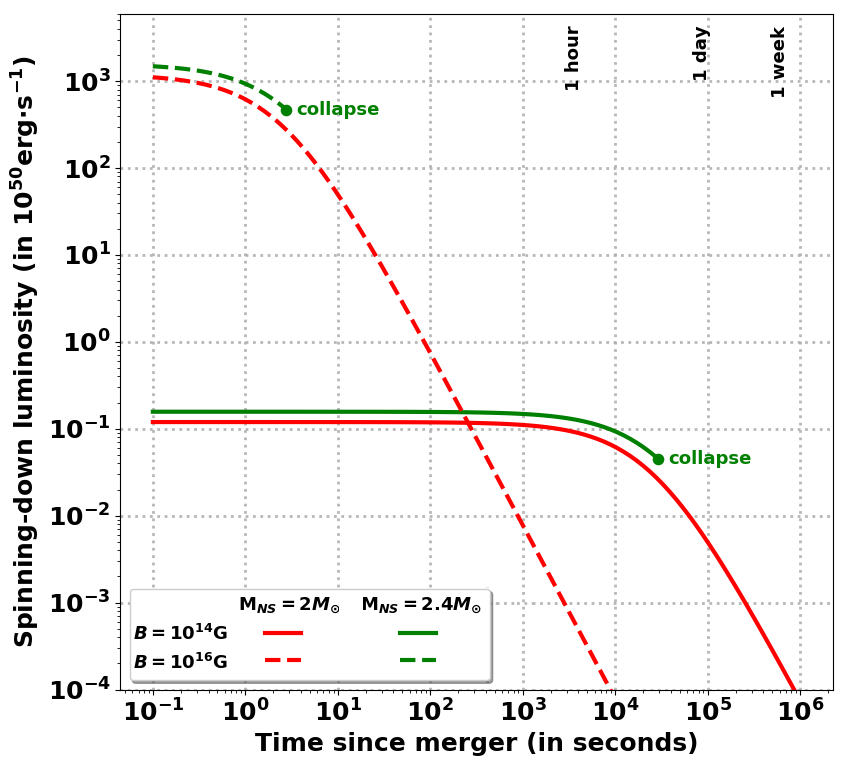
\includegraphics[width=10cm]{Figures/spinning-down_luminosity.png}}
%\vspace*{-0.4cm}
\end{figure}

\section{Fall-back accretion}

Following the merger, expelled matter can fall back onto the compact remnant. In a \bh-\ns merger, provided the \ns is tidally disrupted before it crosses the event horizon, large amounts of material can be ejected in the orbital plane, especially for a stiff \ns \eos such as those favored by the \gw observations of last year double \ns merger. A disc can form and a lanthanide-rich disc wind could develop. Although its properties are significantly different from the ones of the line-driven winds of massive stars, this type of wind could be represented using numerical techniques close to those I worked on with Jon Sundqvist during my postdoctoral years (\eg periodic long characteristics in Cartesian slabs and effective acceleration inhibition distance). In a \ns-\ns merger, the tidally disrupted component co-exists with a quasi-spherical ejecta from the contact interface between the two bodies.

The heating rate of the kilonova due to fall-back accretion can be of the same orders of magnitude as radioactive decay and magnetar spinning-down. Part of the matter falling back might power a collimated ultra-relativistic jet similar to that responsible for the earlier \grb. It has been suggested to account for the long-lived X-ray afterglow observed after the double \ns merger of last year. This highly dynamical phase does require multi-dimensional simulations to disentangle between the intrinsic properties and the contribution of the viewing angle on the observations.

\section{Numerical tool and host institution}

The short \grb and kilonova emission which followed the double \ns merger of last year were particularly unusual. The host galaxy turned out to be an early-type galaxy and the short \grb was faint while the kilonova was luminous and blue. Although unusual, these properties were certainly not marginal as noted by \citet{Troja2018} who identified another pair short \grb\xspace/ kilonova with a similar unexpected behavior. Were they also associated to an undetected double \ns merger? Was the blue color of the kilonova due to the formation of a long-lived \ns whose flux of neutrinos could have inhibited lanthanide nucleosynthesis? Was its high luminosity due to the heating by the central engine? Was the short \grb intrinsically fainter due to the absence of \bh formation \citep{Murguia-Berthier2014,Murguia-Berthier2017a}? Or was it an ultra-relativistic jet seen off-axis? 

Observers have sketched new diagnostics \citep{Gill2018} but their efforts will be wasted if they can not rely on robust numerical results to put their data into perspectives. Typically, the bias introduced by the inclination of the system with respect to our line-of-sight can be alleviated in the incoming years, provided we carry out full 3D numerical simulations. I propose to make use of the finite volume code I have been using and co-developing for the last five years, \texttt{MPI-AMRVAC} (for Message Passing Interface - Adaptive Mesh Refinement Versatile Advection Code), to characterize the geometry of the different components.

During the last decade, numerical simulations have revolutionized the field of core-collapse supernovae and provided an inestimable support to understand long \grbs. They showed how important three-dimensional dynamics and micro-physics (\eg neutrino heating) could be to solve the old conundrum of the stalling shock. Now that compact object mergers are directly within our reach, it is time to deploy the same efforts for short \grbs. High performance computing facilities such as the ones I daily use already exist at the national (\eg CINES and VSC) and European levels to carry out this computational investigation, and so do the massively parallel codes. \texttt{MPI-AMRVAC} provides a versatile environment to solve the equations of \mhd in their conservative form, in a classical or a relativistic framework. 

Efforts at the LUTh by Zakaria Meliani have been made to make \texttt{MPI-AMRVAC} solve the Einstein equations and compute dynamical non-analytic metrics. The LUTh hosts world-leading experts in general relativity and alternative theories of gravity (\eg Laura Bernard and Eric Gourgoulhon) whose knowledge is of tremendous importance to design the numerical schemes appropriate to perform such a computation. Coupling tools like the spectral solver Kadath developed by Philippe Grandcl\'{e}ment to \texttt{MPI-AMRVAC} would lead to a brand new family of codes solving the dynamics of the flow and the metrics all together, a decisive asset in the relativistic environment of a compact object merger. On the other hand, the models of \grb, \ns interior, magnetosphere and micro-physics designed respectively by Fr\'{e}d\'{e}ric Daigne (IAP), J\'{e}r\^{o}me Novak (LUTh), Fabrice Mottez (LUTh) and Micaela Oertel (LUTh) provide a firm semi-analytical bedrock to build upon. These models can make accurate predictions for simplified geometries or in asymptotic regimes which serve to validate numerical setups before running jobs on high performance computing facilities.

\newpage

Many unanswered questions remain and more are to be expected in the next years. The interpretation of the plethora of kilonovae light curves to come requires a better understanding of the Physics at stake now that new constrains are set by the concomitant \gw and \grb observations. Although much uncertainty remains on the exact coalescence rates of \ns-\ns and \bh-\ns binaries, the current and incoming facilites (Advanced LIGO in the US, Advanced Virgo in Europe, KAGRA in Japan and LIGO-India) are expected to detect from a few to one hundred \gw events per year. 

I am willing to take part in this collective effort at LUTh and to bring a numerical expertise suitable to the problems tackled by its members. As my supervision record indicates, I would try to attract excellent Master and PhD candidates to support this effort. Thanks to the Pegasus Marie Sk\l{}odowska-Curie grant I received in 2017, I am also in an ideal position to apply for ERC grants in the following years, in an attempt to provide the necessary momentum to the field of kilonovae and short \grbs in France.




%\phantom{\cite{ElMellah2016a,ElMellah2018a,Xia2017,Rappaport:2012wi,Rappaport2013,SanchisOjeda:2014ww}}
%%\subsubsection*{References}
\vspace*{0.6cm}
\setlength\bibitemsep{0pt}
%%\scriptsize
%\bibliographystyle{ieeetr}
%\bibliography{/Users/Ileyk/Documents/Bibtex/Hubble_fellowship_no_url}

%\settoggle{bbx:url}{false}
%\settoggle{bbx:doi}{false}
%\settoggle{bbx:eprint}{false}
%\bibliographystyle{ieeetr}
%\nocite{MEMSnet,wilde,markey}
\printbibliography[heading=none,title={},omitnumbers=true]


\end{document}
%%%%%%%%%%%%%%%%%  Fin du fichier Latex  %%%%%%%%%%%%%%%%%%%%%%%%%%%%%%

